\chapter{Structured Peer-to-Peer Overlays}
\label{structured_p2p}
Structured P2P systems provide distributed look up services with guaranteed
search time with a lower bound of $O(\log N)$, in contrast to unstructured
systems, which rely on global knowledge/broadcasts, or stochastic techniques
such as random walks~\cite{unstructured_v_structured}.  Some examples of
structured systems can be found in~\cite{pastry, chord, symphony, kademlia,
can, brunet}.  In general, structured systems are able to make these guarantees
by self-organizing a structured topology, such as a 2D ring (pictured in
Figure~\ref{fig:ring_overlay} or a hypercube.  Joining an overlay usually
follows some form of these abstracted steps:
\begin{enumerate}
\item generate or obtain a unique identification number (node ID) on the
order of 128-bits to 256-bits,
\item connect to random addresses on a pre-shared well-known endpoints list,
\item becomes connected to at least one peer in the list (leaf connection),
\item find the peers closest in the address space to the selected node ID,
\item connect to nodes whose IDs are immediately smaller and / or larger than
its (neighbor connections),
\item and finally connect to other nodes in the overlay that are not local in
the address space (shortcut connections).
\end{enumerate}

Each node must have a unique node ID, address collisions can prevent nodes from
participating in the overlay and can potentially fragment overlays preventing
them from working properly.  Having node IDs well distributed assists in
providing better scalability in structured overlays routing enabling fewer
shortcut connections due to the uniformly distributed nature of the system.
Each node can generate their own address if they use a cryptographically strong
random number generator.  Another approach for distributing node IDs relies
using a trusted third party to generate node IDs and cryptographically sign
them~\cite{secure_routing}.

Depending on the protocol, a node must be connected to closest neighbors in the
node ID address space; optimizations for fault tolerance suggest that for ring
topologies the amount should be between 2 to $\log(N)$ on both sides.  In the
case of overlay disconnectivity especially when related to churn, when a peer
does not know the address of its immediate predecessor or successor and a
message is routed through it destined for them, depending on the message type,
it may either be locally consumed or thrown away, never arriving at its
intended destination.  Having multiple neighbors assists in stabilizing the
overlay structure when experiencing churn, particularly when peers leave 
suddenly without warning.

Overlay shortcuts enable efficient routing in ring-structured P2P systems.  The
different shortcut selection methods include: maintaining large tables without
using connections and only verifying usability when routing
messages~\cite{pastry, kademlia}, maintaining a connection with a peer every
set distance in the P2P address space~\cite{chord}, or using locations drawn
from a harmonic distribution in the node address space~\cite{symphony}.

Most structured P2P overlays support decentralized storage/look-up of information by
mapping keys to specific node IDs in an overlay.  At a minimum, the data is stored
at the node ID either smaller or larger to the data's node ID and for fault
tolerance the data can be stored at other nodes.  This sort of mapping
and data storage is called a distributed hash table (DHT).  DHTs provide the
building blocks to form more complex distributed data stores as presented in
Past~\cite{past} and Kosha~\cite{kosha}.

There are two mechanisms for message routing in a P2P overlay: iterative or
recursive.  In iterative routing, the sender of a packet will directly contact
each successive member in a path querying it for the next until arriving at the
destination node, sending the packet directly to the destination.  In recursive
routing, messages are sent through the overlay via forwarding from one peer to
the next until arriving at the destination.  In general, iterative routing is
easier to implement though comes with considerable overhead as each overlay
query will cause $\log(N)$ connections to form and makes NAT traversal
complicated as it will require constant traversal mediation and need to be made
quickly, whereas recursive routing provides stable connections due to a single
NAT traversal during the connection phase.

\section{Network Address Translation Hampering P2P Systems}
As of 2009, the majority of the Internet is connected via Internet Protocol (IP)
version 4.  A limitation in this protocol is that there are only $2^{32}$
addresses total though or approximately 4 billion addresses.  With the
Earth already having a population of over 8 billion and each individual having
multiple devices that have Internet connectivity the IPv4 limitation is becoming
more and more apparent.  IPv6 provides an alternative, supporting $2^{128}$
addresses, it is not pervasive with only X\% of the Internet reachable via IPv6. 
In the meantime during the transition from IPv4 to IPv6, network address
translation (NAT) enables many machines and devices to share a single IP
address.  The cost of this operation means that such machines lose direct
addressability on the Internet.

When a machine, \textit{A}, behind a typical NAT, \textit{B}, sends out a
packet to an Internet host, \textit{C}, the NAT box translates the packet so
that it appears it is coming from the NAT device making the NAT box a gateway.
When the the packet is sent from \textit{A} to \textit{C}, the source and
destination are listed as IP, port pairs, where the source and destination are
$IP_A:Port_A$ and $IP_C:Port_C$, respectively.  \textit{A} forwards the packet
to \textit{B} who transforms the source from $IP_A:Port_A$ to $IP_B:Port_B$,
where $Port_A$ may or may not be equal to $Port_B$.  This creates a NAT mapping
so that incoming packets from $IP_C:Port_C$ to $IP_B:Port_B$ are translated and
forwarded to $IP_A:Port_A$.

There are a handful of recognized NAT devices as presented in~\cite{stun,
p2p_nats_rfc}.  The following list focuses on the more prevalent types:
\begin{itemize}
\item full cone - all requests from the same internal IP and port are mapped to
a static external IP and port, thus any external host can communicate with the
internal host once a mapping has been made,
\item restricted cone - like a full cone but requires that the internal host
has sent a message to the external host before the NAT will pass the packets,
\item port restricted cone - like a restricted cone but requires that the
internal host has sent the packet to the external hosts specific port before the
NAT will pass packets,
\item symmetric - each source and destination pair have no relation, thus only
a machine receiving a message from an internal host can send a message back.
\end{itemize}

Peers on cone NATs can easily be traversed so long as a third party assists in
determining the port allocated by the NAT and they exchange NAT penetration
messages.  Peers behind symmetric NATs cannot easily communicate with each
other, since there is no relation between remote hosts and ports and local
ports.  Further complicating the matter is that there are various types of
symmetric NATs, having behaviors similar to full, restricted, and port
restricted cone NATs.  \cite{nat_stun} describes methods to traverse these
NATs so long as there is a predictable pattern to port selection.  In general,
these approaches use UDP because of the lack of additional protocol states,
that require replay and ignoring reject methods that occur with the TCP
handshake,  though there is reasonable amount of work describing TCP NAT
traversal such as~\cite{tcp_nat}.  TCP NAT traversal is complicated by stateful
firewalls, or those that watch connections and connection attempts preventing
messages from closed TCP channels from passing through the NAT.  For NAT
situations that cannont be traversed, a third party can act as a relay between
the two, this is known as triangulation or traversal using relay NAT (TURN),
described in~\cite{turn}.

\subsection{NAT Traversal in Structured Overlays}
Structured overlays rely on the principle that any peer can become directly
connected with any other peer in the system.  Thus in order to use structured
overlays on the Internet, they must either be run on publicly accessable
addresses or support NAT traversal.  Even in the case where there is NAT
traversal, occassionally there are Internet routing table breaks and two
peers who should be able to directly communicate cannot.

To date, there exists only one solution, Brunet~\cite{brunet}, supporting
decentralized UDP NAT traversal and limited relays.  To support UDP NAT
traversal, Brunet makes connection attempts bidirectional with peers exchange
all known IP addresses and ports, which it knows directly and from external
overlay nodes.  This enables the traversal of all forms of cone NATs, but
symmetric NATs require iterative rounds of traversal attempts and cannot be
traversed.  If two peers cannot connect, they exchange list of peers, if an
overlap exists, they will forward packets through it to each
other~\cite{hpdc08_1}, this approach was used to ensure the structure of
the overlay and cannot be used to form arbitrary relay connections.  To address
this as my interest lie in forming efficient VPNs, I have designed a technique
that causes peers to proactively creates overlap and when multiple overlap
exist to route through the most attractive candidate, as represeted in
Figure~\ref{fig:relay}.

To assist in the selection of overlap connection, peers exchange arbitrary
information along with the neighbor lists.  So far I have implemented systems
that share information about node stability (measured by the age of a
connection) and proximity (based upon ping latency to neighbors).  When overlap
changes, peers can select to use only a subset of the overlap, thus only the
fastest or most stable peers are used with extras in reserve.

\subsection{Usefulness of Relays}
To verify the usefulness of two-hop over overlay routing, I have evaluted
the latency approach using an event-driven simulator that reuses the code
base of IPOP to faithfully implement its functionality using event-driven
simulated times to emulate WAN latencies.  For this experiment, I chose
latencies based upon the MIT King Data Set~\cite{king_data}, which consists of
all-to-all latencies between 1,740 well-distributed Internet hosts.  We
then evaluated overlays using various network sizes up to 1,740.  After
starting the overlay and the system reaches steady state, that is the overlay
is completely formed and no new connections are created, I measured
the average all-to-all latency for all messages that would have taken two
overlay hops or more, the average of the low latency relay model, and the
average of single hop communication.  In the low latency relay model, each
destination node form a connection to the source node's physically closest peer
as determined via latency (in a live system by application level ping).  Then
this pathway is used as a two-hop relay between source and node.  We only look
at two overlay hops and more, as a single hop would only benefit under
triangular inequalities that are not a consideration in my work.  

The results are presented in Figure~\ref{fig:simulated_relays}.  I performed
the tests for varying network sizes.  Tests began with network sizes of 25, 
sizes around 20 and under tend to be fully connected due to the connectivity
requirements of the system.  It is not until the network size expands past 100
and towards 200 nodes that relays become significantly beneficial.  At
100 nodes, there is approximately a 54\% performance increase, whereas at
200 there is an 87\% increase and it appears to grow proportionately to the size
of the pool.  The key take away is that latency-bound applications
using a reasonably sized overlay would significantly benefit from
the use of two-hop relays.

\section{Using Structured Overlays for Direct Communication}
Applications like VPNs, games, media, and communication can benefit from using
an overlay for discovery and limited communication, though as communication
increases in frequency direct communication may be perferred.  In previous
work~\cite{wow}, the authors describe a method for transparently detecting this
behavior and creating direct links as a result.  In comparing a VPN built on
top of an overlay with a point-to-point direct approach, the VPN using the
overlay has significant overheads due to each IP packet traversing the overlays
state machine prior to being sent to the VPN.  Thus for high bandwidth
applications, this approach does not scale and costs significant CPU
utilization.

To address this issue, I propose two models in addition to the existing
approach to using an overlay for high bandwidth purposes.  These two
approaches are:  1) use the structured overlay to create and maintain
links but placing the application between the connection and the overlay
stack so that the application has first access to the data and 2) use
the structured overlay to discover peers but the application creates and
manages its own links using the structured overlay to coordinate these
efforts.  The proposed approaches are presented in
Figure~\ref{fig:direct_communication}.

The first approach benefits from using existing components of the structured
overlay including link creation and maintenance though may still have overheads
due to packets needing to traverse both the application and overlays stack.
This can be addressed by creating a unique thread for processing packets in the
application as well as the overlay stacks.  Since the connections are shared,
this approach will require additional thread sychronization.

The second approach is more complex but both components reside in completely
different memory spaces.  The application might be easily coded through code
reuse, but this still significantly increases the complexity of the solutions.
Because the stacks each component has its own stack, there is no need to
handle synchronization.  The VPN will have unfettered access to the connections
it has established.

\section{Overlay-Aware TCP}
When sending a message via an overlay, if a packet is lost in transit, there
are no built-in methods for recovering the transmission, the overlay acts like
a datagram system.  Even when links are connected by TCP, a disconnectivity
or failure in the overlay will not trigger successful TCP transmissions to
transmit the packet to another host.  When using UDP, there are no built-in
methods.  Current approaches either fail or attempt a simple retry mechanism.
Even in the case of retrying, UDP does not handle fragmentation well and to
support retrying either requires complicated state to handle large packets
or a simple state that cannot support large packets.  I implement an overlay
TCP system and use it in real system to determine other challenges that exist
when using it.

\section{Figures and Tables}

\begin{figure}[ht]
\centering
%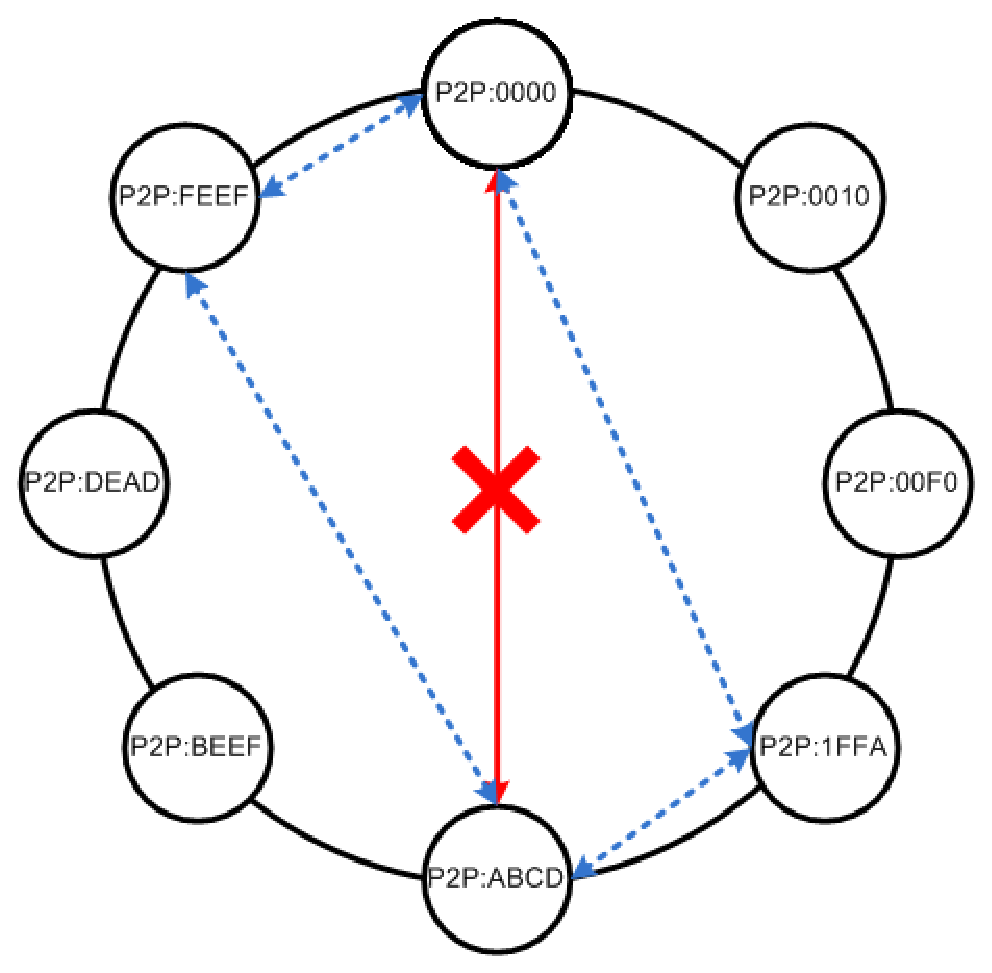
\epsfig{file=figs/relay.png.eps}
\caption{1-D Ring Structured Overlay}
\label{fig:ring_overlay}
\end{figure}

\begin{figure}[ht]
\centering
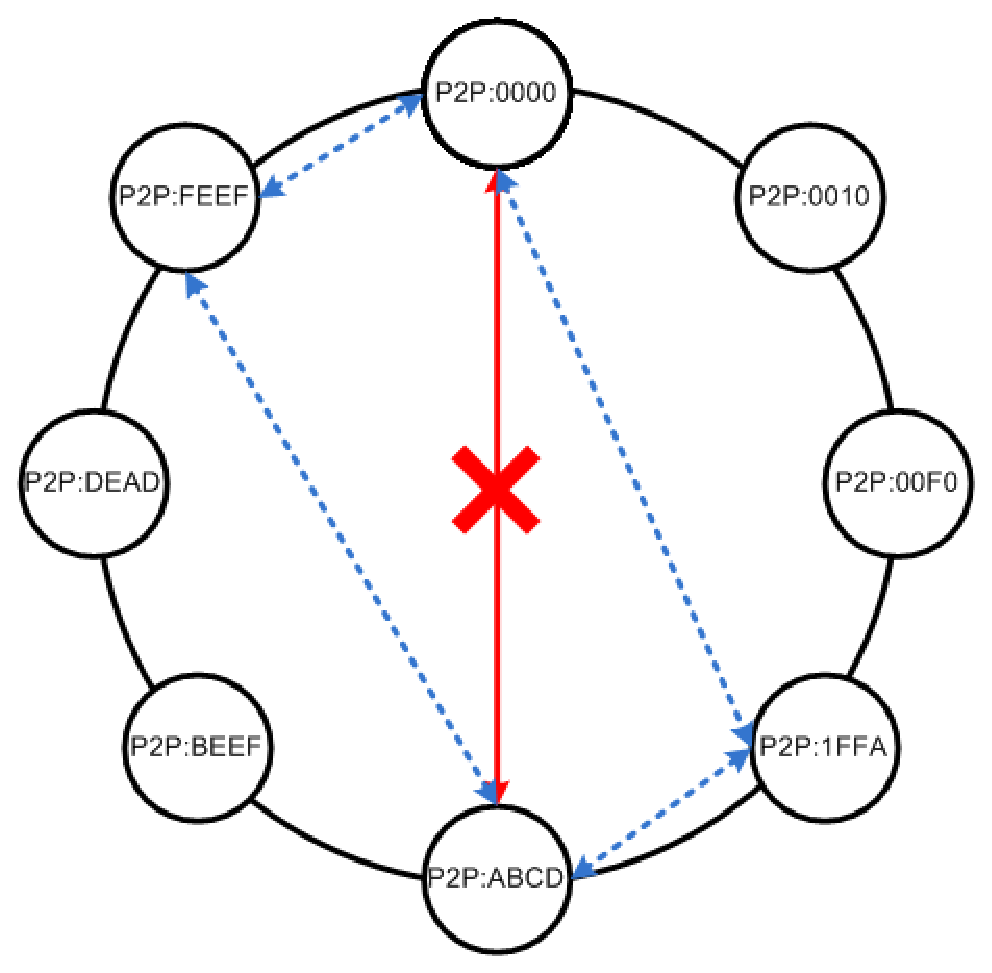
\epsfig{file=figs/relay.png.eps, width=4in}
\caption[Proactive relay creation]{Creating relays across the node address
space, when direct connectivity is not possible.  Two members, 0000 and ABCD, 
desire a direct connection but are unable to directly connect, perhaps due to
NATs or firewalls.  They exchange neighbor information through the overlay and
connect to one of each other's neighbors, creating an overlap.  The overlap
then becomes a relay path (represented by dashed lines), improving performance
over routing across the entire overlay.}
\label{fig:relay}
\end{figure}

\begin{figure}[ht]
\centering
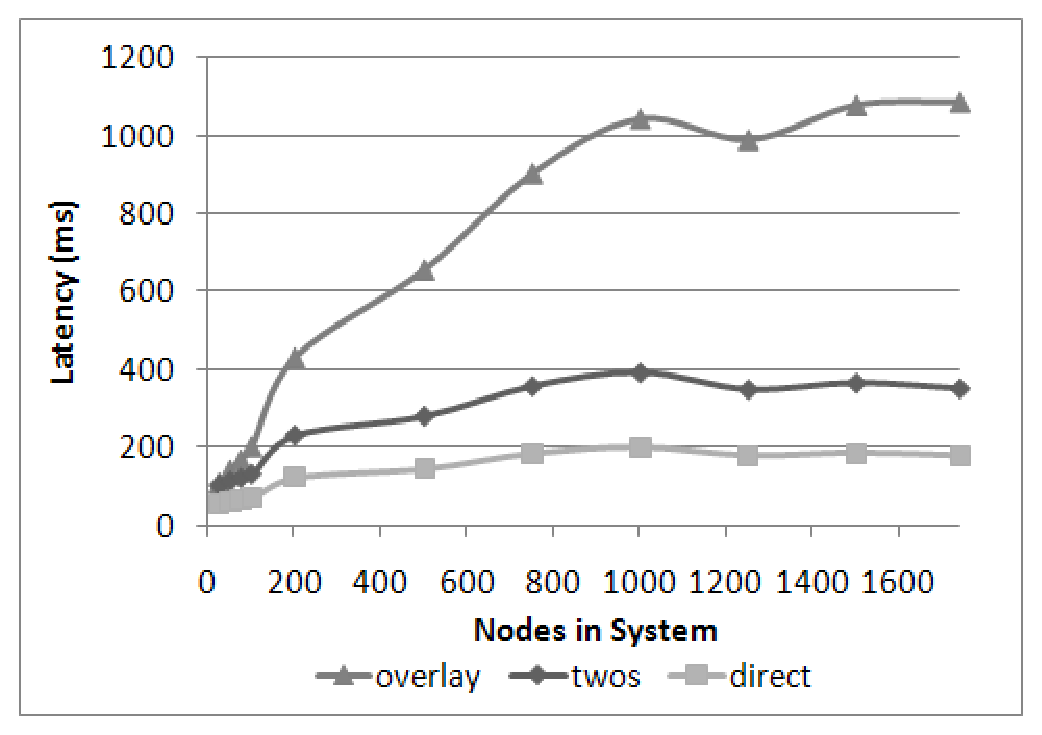
\epsfig{file=figs/relay_motivation.png.eps, width=4in}
\caption[Relay evaluation]{A comparison of the average all-to-all overlay
routing, two-hop relay, and direct connection latency in a Structured P2P
environment, Brunet, using the King data set.}
\label{fig:simulated_relays}
\end{figure}

\begin{figure}[ht]
\centering
\caption{Direct communication models}
\label{fig:direct_communication}
\end{figure}
